\documentclass[12pt,a4paper]{article}
\usepackage[margin=0.8cm,landscape]{geometry}
\usepackage{tikz}
\usetikzlibrary{positioning, shapes.geometric, arrows.meta, calc}
\usepackage{xcolor}
\usepackage{booktabs}
\usepackage{longtable}

% Define colors - clean and clear
\definecolor{networkbox}{RGB}{255, 240, 245}
\definecolor{networktext}{RGB}{0, 0, 0}
\definecolor{linkcolor}{RGB}{100, 100, 100}
\definecolor{highlight}{RGB}{255, 200, 220}
\definecolor{routercolor}{RGB}{220, 255, 220}
\definecolor{branchcolor}{RGB}{240, 255, 240}

\tikzset{
    network node/.style={
        rectangle,
        rounded corners=3pt,
        draw=networktext,
        fill=networkbox,
        text width=2.8cm,
        text centered,
        minimum height=1cm,
        font=\tiny,
        inner sep=3pt,
        align=center
    },
    leaf node/.style={
        rectangle,
        rounded corners=3pt,
        draw=networktext,
        fill=highlight,
        text width=2.8cm,
        text centered,
        minimum height=1cm,
        font=\tiny,
        inner sep=3pt,
        align=center
    },
    router node/.style={
        rectangle,
        rounded corners=3pt,
        draw=networktext,
        fill=routercolor,
        text width=2.5cm,
        text centered,
        minimum height=0.9cm,
        font=\tiny,
        inner sep=2pt,
        align=center
    },
    branch node/.style={
        rectangle,
        rounded corners=3pt,
        draw=networktext,
        fill=branchcolor,
        text width=2.8cm,
        text centered,
        minimum height=1cm,
        font=\tiny,
        inner sep=3pt,
        align=center
    },
    connection/.style={
        -,
        color=linkcolor,
        line width=0.6pt
    }
}

\begin{document}
\pagestyle{empty}

\begin{center}
\Large\textbf{VLSM Subnetting Tree Diagram}\\
\vspace{0.3cm}
\small ROOT SUPERNET: 100.160.0.0/12\\
\small Range: 100.160.0.0 - 100.175.255.255
\end{center}

\vspace{0.5cm}

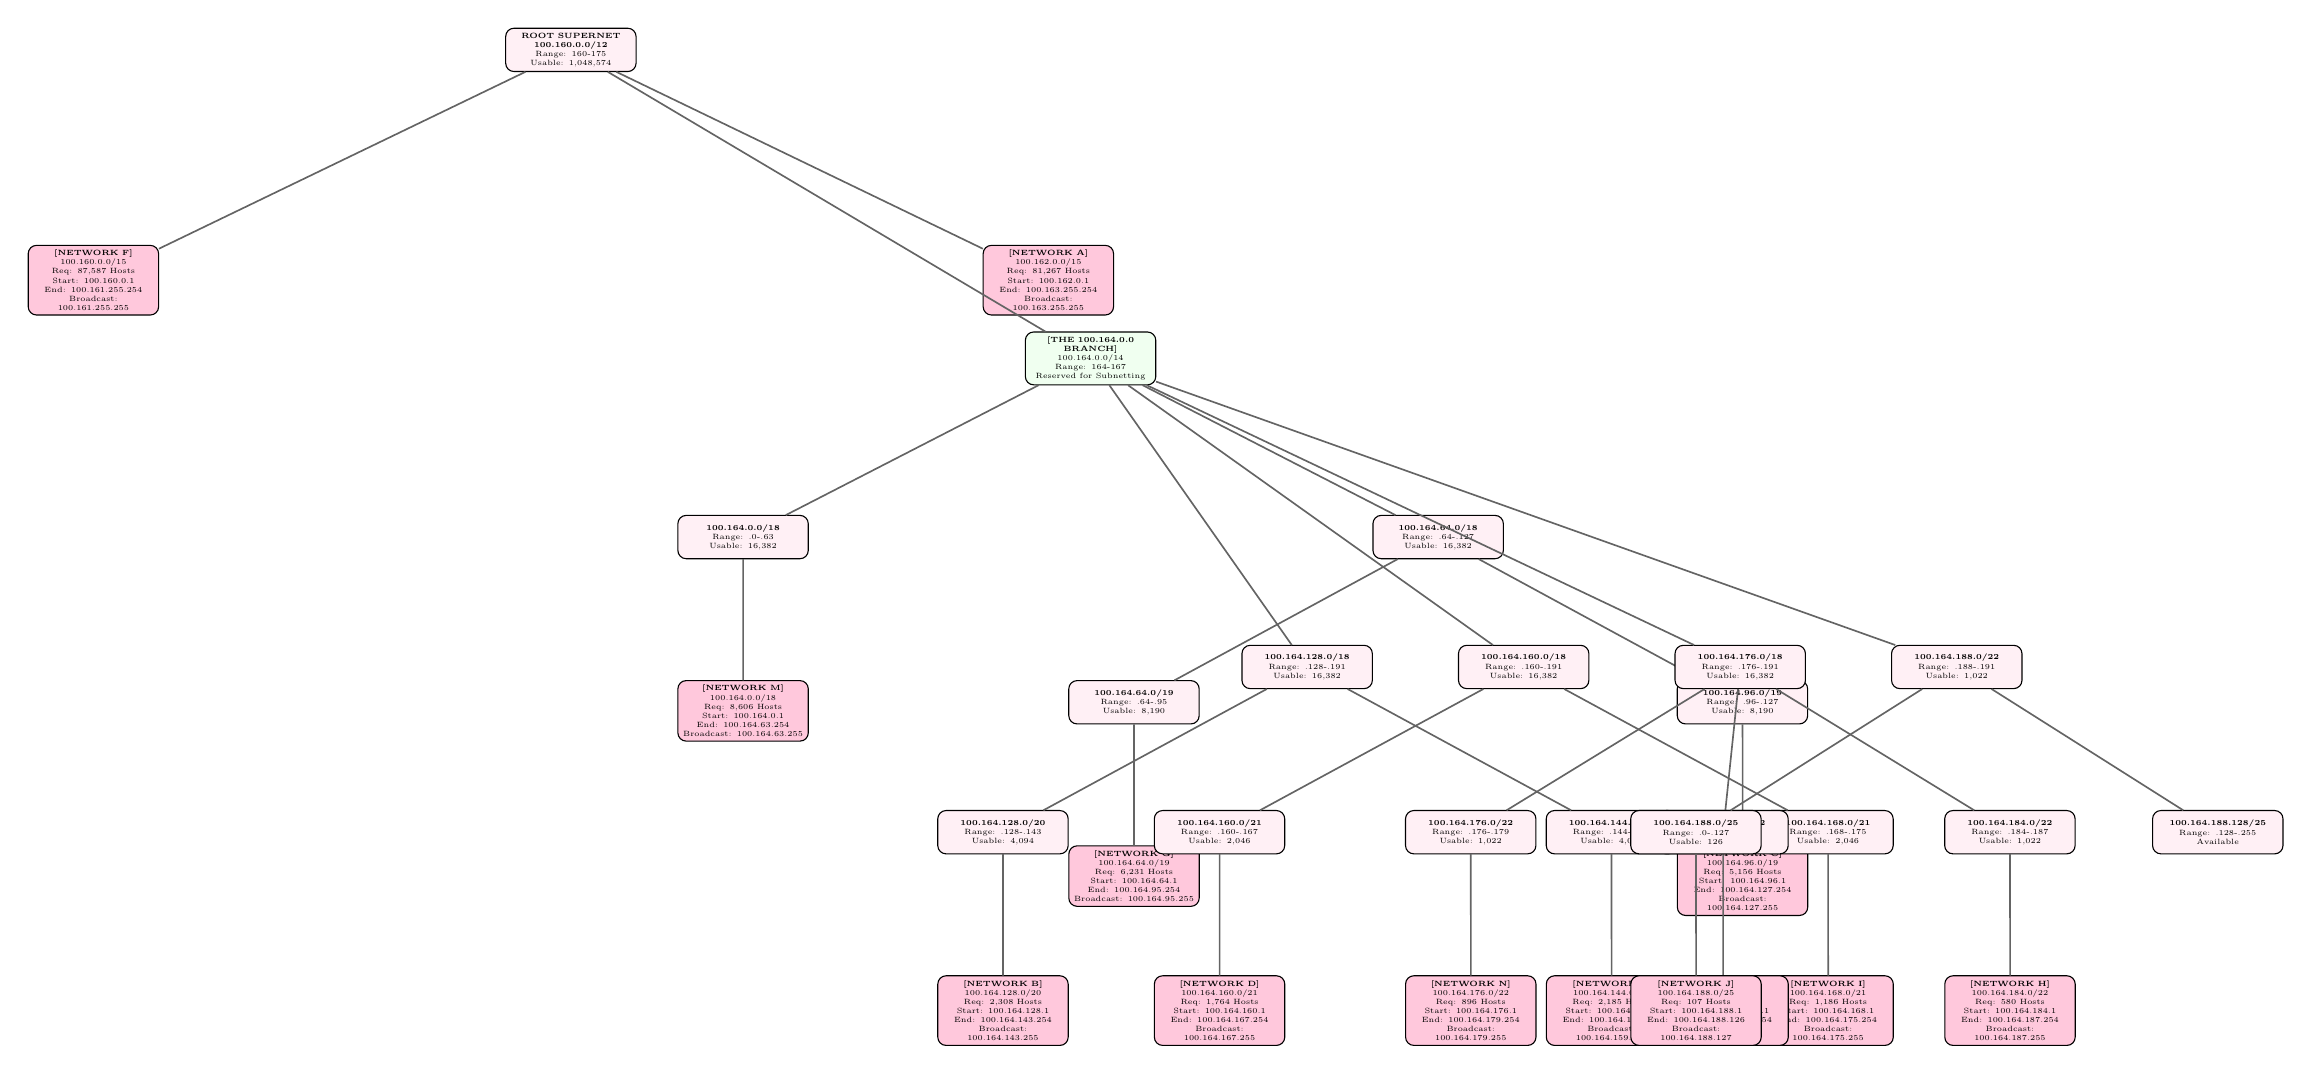
\begin{tikzpicture}[
    node distance=2.8cm and 6cm,
    scale=0.55,
    transform shape
]

% ============================================
% ROOT LEVEL: Base Network 100.160.0.0/12
% ============================================
\node[network node] (root) at (0,0) {
    \textbf{ROOT SUPERNET}\\
    \textbf{100.160.0.0/12}\\
    Range: 160-175\\
    Usable: 1,048,574
};

% ============================================
% LEVEL 1: Network F (100.160.0.0/15)
% ============================================
\node[leaf node, below left=4cm and 8cm of root] (netF) {
    \textbf{[NETWORK F]}\\
    100.160.0.0/15\\
    Req: 87,587 Hosts\\
    Start: 100.160.0.1\\
    End: 100.161.255.254\\
    Broadcast: 100.161.255.255
};

\draw[connection] (root) -- (netF);

% ============================================
% LEVEL 1: Network A (100.162.0.0/15)
% ============================================
\node[leaf node, below right=4cm and 8cm of root] (netA) {
    \textbf{[NETWORK A]}\\
    100.162.0.0/15\\
    Req: 81,267 Hosts\\
    Start: 100.162.0.1\\
    End: 100.163.255.254\\
    Broadcast: 100.163.255.255
};

\draw[connection] (root) -- (netA);

% ============================================
% LEVEL 1: The 100.164.0.0 Branch (/14 continuation)
% ============================================
\node[branch node, below=6cm of root, xshift=12cm] (branch_164) {
    \textbf{[THE 100.164.0.0 BRANCH]}\\
    100.164.0.0/14\\
    Range: 164-167\\
    Reserved for Subnetting
};

\draw[connection] (root) -- (branch_164);

% ============================================
% LEVEL 2: Split 100.164.0.0/14 into /18
% ============================================
\node[network node, below left=3cm and 5cm of branch_164] (l2_0) {
    \textbf{100.164.0.0/18}\\
    Range: .0-.63\\
    Usable: 16,382
};

\node[network node, below right=3cm and 5cm of branch_164] (l2_64) {
    \textbf{100.164.64.0/18}\\
    Range: .64-.127\\
    Usable: 16,382
};

\draw[connection] (branch_164) -- (l2_0);
\draw[connection] (branch_164) -- (l2_64);

% ============================================
% LEVEL 3: Network M (from 100.164.0.0/18)
% ============================================
\node[leaf node, below=2.8cm of l2_0] (netM) {
    \textbf{[NETWORK M]}\\
    100.164.0.0/18\\
    Req: 8,606 Hosts\\
    Start: 100.164.0.1\\
    End: 100.164.63.254\\
    Broadcast: 100.164.63.255
};

\draw[connection] (l2_0) -- (netM);

% ============================================
% LEVEL 3: Split 100.164.64.0/18 into /19
% ============================================
\node[network node, below left=2.8cm and 4cm of l2_64] (l3_64) {
    \textbf{100.164.64.0/19}\\
    Range: .64-.95\\
    Usable: 8,190
};

\node[network node, below right=2.8cm and 4cm of l2_64] (l3_96) {
    \textbf{100.164.96.0/19}\\
    Range: .96-.127\\
    Usable: 8,190
};

\draw[connection] (l2_64) -- (l3_64);
\draw[connection] (l2_64) -- (l3_96);

% ============================================
% LEVEL 4: Networks G and C
% ============================================
\node[leaf node, below=2.8cm of l3_64] (netG) {
    \textbf{[NETWORK G]}\\
    100.164.64.0/19\\
    Req: 6,231 Hosts\\
    Start: 100.164.64.1\\
    End: 100.164.95.254\\
    Broadcast: 100.164.95.255
};

\node[leaf node, below=2.8cm of l3_96] (netC) {
    \textbf{[NETWORK C]}\\
    100.164.96.0/19\\
    Req: 5,156 Hosts\\
    Start: 100.164.96.1\\
    End: 100.164.127.254\\
    Broadcast: 100.164.127.255
};

\draw[connection] (l3_64) -- (netG);
\draw[connection] (l3_96) -- (netC);

% ============================================
% LEVEL 2: Continue with 100.164.128.0/18
% ============================================
\node[network node, below=6cm of branch_164, xshift=5cm] (l2_128) {
    \textbf{100.164.128.0/18}\\
    Range: .128-.191\\
    Usable: 16,382
};

\draw[connection] (branch_164) -- (l2_128);

% ============================================
% LEVEL 3: Split 100.164.128.0/18 into /20
% ============================================
\node[network node, below left=2.8cm and 4cm of l2_128] (l3_128) {
    \textbf{100.164.128.0/20}\\
    Range: .128-.143\\
    Usable: 4,094
};

\node[network node, below right=2.8cm and 4cm of l2_128] (l3_144) {
    \textbf{100.164.144.0/20}\\
    Range: .144-.159\\
    Usable: 4,094
};

\draw[connection] (l2_128) -- (l3_128);
\draw[connection] (l2_128) -- (l3_144);

% ============================================
% LEVEL 4: Networks B and L
% ============================================
\node[leaf node, below=2.8cm of l3_128] (netB) {
    \textbf{[NETWORK B]}\\
    100.164.128.0/20\\
    Req: 2,308 Hosts\\
    Start: 100.164.128.1\\
    End: 100.164.143.254\\
    Broadcast: 100.164.143.255
};

\node[leaf node, below=2.8cm of l3_144] (netL) {
    \textbf{[NETWORK L]}\\
    100.164.144.0/20\\
    Req: 2,185 Hosts\\
    Start: 100.164.144.1\\
    End: 100.164.159.254\\
    Broadcast: 100.164.159.255
};

\draw[connection] (l3_128) -- (netB);
\draw[connection] (l3_144) -- (netL);

% ============================================
% LEVEL 3: Continue with 100.164.160.0/18
% ============================================
\node[network node, below=6cm of branch_164, xshift=10cm] (l3_160) {
    \textbf{100.164.160.0/18}\\
    Range: .160-.191\\
    Usable: 16,382
};

\draw[connection] (branch_164) -- (l3_160);

% ============================================
% LEVEL 4: Split 100.164.160.0/18 into /21
% ============================================
\node[network node, below left=2.8cm and 4cm of l3_160] (l4_160) {
    \textbf{100.164.160.0/21}\\
    Range: .160-.167\\
    Usable: 2,046
};

\node[network node, below right=2.8cm and 4cm of l3_160] (l4_168) {
    \textbf{100.164.168.0/21}\\
    Range: .168-.175\\
    Usable: 2,046
};

\draw[connection] (l3_160) -- (l4_160);
\draw[connection] (l3_160) -- (l4_168);

% ============================================
% LEVEL 5: Networks D and I
% ============================================
\node[leaf node, below=2.8cm of l4_160] (netD) {
    \textbf{[NETWORK D]}\\
    100.164.160.0/21\\
    Req: 1,764 Hosts\\
    Start: 100.164.160.1\\
    End: 100.164.167.254\\
    Broadcast: 100.164.167.255
};

\node[leaf node, below=2.8cm of l4_168] (netI) {
    \textbf{[NETWORK I]}\\
    100.164.168.0/21\\
    Req: 1,186 Hosts\\
    Start: 100.164.168.1\\
    End: 100.164.175.254\\
    Broadcast: 100.164.175.255
};

\draw[connection] (l4_160) -- (netD);
\draw[connection] (l4_168) -- (netI);

% ============================================
% LEVEL 4: Continue with 100.164.176.0/18
% ============================================
\node[network node, below=6cm of branch_164, xshift=15cm] (l4_176) {
    \textbf{100.164.176.0/18}\\
    Range: .176-.191\\
    Usable: 16,382
};

\draw[connection] (branch_164) -- (l4_176);

% ============================================
% LEVEL 5: Split into /22 networks
% ============================================
\node[network node, below left=2.8cm and 3.2cm of l4_176] (l5_176) {
    \textbf{100.164.176.0/22}\\
    Range: .176-.179\\
    Usable: 1,022
};

\node[network node, below=2.8cm of l4_176, xshift=-0.4cm] (l5_180) {
    \textbf{100.164.180.0/22}\\
    Range: .180-.183\\
    Usable: 1,022
};

\node[network node, below right=2.8cm and 3.2cm of l4_176] (l5_184) {
    \textbf{100.164.184.0/22}\\
    Range: .184-.187\\
    Usable: 1,022
};

\draw[connection] (l4_176) -- (l5_176);
\draw[connection] (l4_176) -- (l5_180);
\draw[connection] (l4_176) -- (l5_184);

% ============================================
% LEVEL 6: Networks N, E, and H
% ============================================
\node[leaf node, below=2.8cm of l5_176] (netN) {
    \textbf{[NETWORK N]}\\
    100.164.176.0/22\\
    Req: 896 Hosts\\
    Start: 100.164.176.1\\
    End: 100.164.179.254\\
    Broadcast: 100.164.179.255
};

\node[leaf node, below=2.8cm of l5_180] (netE) {
    \textbf{[NETWORK E]}\\
    100.164.180.0/22\\
    Req: 810 Hosts\\
    Start: 100.164.180.1\\
    End: 100.164.183.254\\
    Broadcast: 100.164.183.255
};

\node[leaf node, below=2.8cm of l5_184] (netH) {
    \textbf{[NETWORK H]}\\
    100.164.184.0/22\\
    Req: 580 Hosts\\
    Start: 100.164.184.1\\
    End: 100.164.187.254\\
    Broadcast: 100.164.187.255
};

\draw[connection] (l5_176) -- (netN);
\draw[connection] (l5_180) -- (netE);
\draw[connection] (l5_184) -- (netH);

% ============================================
% LEVEL 5: Final Network J (/25)
% ============================================
\node[network node, below=6cm of branch_164, xshift=20cm] (l5_188) {
    \textbf{100.164.188.0/22}\\
    Range: .188-.191\\
    Usable: 1,022
};

\draw[connection] (branch_164) -- (l5_188);

\node[network node, below left=2.8cm and 3cm of l5_188] (l6_188) {
    \textbf{100.164.188.0/25}\\
    Range: .0-.127\\
    Usable: 126
};

\draw[connection] (l5_188) -- (l6_188);

\node[leaf node, below=2.8cm of l6_188] (netJ) {
    \textbf{[NETWORK J]}\\
    100.164.188.0/25\\
    Req: 107 Hosts\\
    Start: 100.164.188.1\\
    End: 100.164.188.126\\
    Broadcast: 100.164.188.127
};

\draw[connection] (l6_188) -- (netJ);

\node[network node, below right=2.8cm and 3cm of l5_188] (remaining) {
    \textbf{100.164.188.128/25}\\
    Range: .128-.255\\
    Available
};

\draw[connection] (l5_188) -- (remaining);

\end{tikzpicture}

\newpage

% ============================================
% DETAILED NETWORK SUMMARY TABLE
% ============================================
\section*{Complete Network Allocation Summary}

\begin{table}[h]
\centering
\footnotesize
\begin{tabular}{|c|c|c|c|c|c|c|}
\hline
\textbf{Network} & \textbf{Network Address} & \textbf{CIDR} & \textbf{Required Hosts} & \textbf{Usable Hosts} & \textbf{Subnet Mask} & \textbf{Broadcast} \\
\hline
F & 100.160.0.0 & /15 & 87,587 & 131,070 & 255.254.0.0 & 100.161.255.255 \\
A & 100.162.0.0 & /15 & 81,267 & 131,070 & 255.254.0.0 & 100.163.255.255 \\
M & 100.164.0.0 & /18 & 8,606 & 16,382 & 255.255.192.0 & 100.164.63.255 \\
G & 100.164.64.0 & /19 & 6,231 & 8,190 & 255.255.224.0 & 100.164.95.255 \\
C & 100.164.96.0 & /19 & 5,156 & 8,190 & 255.255.224.0 & 100.164.127.255 \\
B & 100.164.128.0 & /20 & 2,308 & 4,094 & 255.255.240.0 & 100.164.143.255 \\
L & 100.164.144.0 & /20 & 2,185 & 4,094 & 255.255.240.0 & 100.164.159.255 \\
D & 100.164.160.0 & /21 & 1,764 & 2,046 & 255.255.248.0 & 100.164.167.255 \\
I & 100.164.168.0 & /21 & 1,186 & 2,046 & 255.255.248.0 & 100.164.175.255 \\
N & 100.164.176.0 & /22 & 896 & 1,022 & 255.255.252.0 & 100.164.179.255 \\
E & 100.164.180.0 & /22 & 810 & 1,022 & 255.255.252.0 & 100.164.183.255 \\
H & 100.164.184.0 & /22 & 580 & 1,022 & 255.255.252.0 & 100.164.187.255 \\
J & 100.164.188.0 & /25 & 107 & 126 & 255.255.255.128 & 100.164.188.127 \\
\hline
\end{tabular}
\caption{All Network Subnets with Complete Details}
\end{table}

\vspace{0.5cm}

\section*{IP Address Range Details}

\begin{table}[h]
\centering
\footnotesize
\begin{tabular}{|c|c|c|c|}
\hline
\textbf{Network} & \textbf{Start IP} & \textbf{End IP} & \textbf{Broadcast Address} \\
\hline
F & 100.160.0.1 & 100.161.255.254 & 100.161.255.255 \\
A & 100.162.0.1 & 100.163.255.254 & 100.163.255.255 \\
M & 100.164.0.1 & 100.164.63.254 & 100.164.63.255 \\
G & 100.164.64.1 & 100.164.95.254 & 100.164.95.255 \\
C & 100.164.96.1 & 100.164.127.254 & 100.164.127.255 \\
B & 100.164.128.1 & 100.164.143.254 & 100.164.143.255 \\
L & 100.164.144.1 & 100.164.159.254 & 100.164.159.255 \\
D & 100.164.160.1 & 100.164.167.254 & 100.164.167.255 \\
I & 100.164.168.1 & 100.164.175.254 & 100.164.175.255 \\
N & 100.164.176.1 & 100.164.179.254 & 100.164.179.255 \\
E & 100.164.180.1 & 100.164.183.254 & 100.164.183.255 \\
H & 100.164.184.1 & 100.164.187.254 & 100.164.187.255 \\
J & 100.164.188.1 & 100.164.188.126 & 100.164.188.127 \\
\hline
\end{tabular}
\caption{Complete IP Address Range for Each Network}
\end{table}

\vspace{0.5cm}

\section*{Router Interface and DHCP Configuration}

\begin{table}[h]
\centering
\footnotesize
\begin{tabular}{|c|c|c|}
\hline
\textbf{Network} & \textbf{Router Interface IP} & \textbf{DHCP Start Range} \\
\hline
F & 100.160.0.1 & 100.160.0.2 \\
A & 100.162.0.1 & 100.162.0.2 \\
M & 100.164.0.1 & 100.164.0.2 \\
G & 100.164.64.1 & 100.164.64.2 \\
C & 100.164.96.1 & 100.164.96.2 \\
B & 100.164.128.1 & 100.164.128.2 \\
L & 100.164.144.1 & 100.164.144.2 \\
D & 100.164.160.1 & 100.164.160.2 \\
I & 100.164.168.1 & 100.164.168.2 \\
N & 100.164.176.1 & 100.164.176.2 \\
E & 100.164.180.1 & 100.164.180.2 \\
H & 100.164.184.1 & 100.164.184.2 \\
J & 100.164.188.1 & 100.164.188.2 \\
\hline
\end{tabular}
\caption{Router Interface and DHCP Pool Configuration}
\end{table}

\vspace{0.5cm}

\section*{Network Utilization Summary}

\begin{table}[h]
\centering
\footnotesize
\begin{tabular}{|c|c|c|c|}
\hline
\textbf{Network} & \textbf{Required Hosts} & \textbf{Usable Hosts} & \textbf{Utilization (\%)} \\
\hline
F & 87,587 & 131,070 & 66.8\% \\
A & 81,267 & 131,070 & 62.0\% \\
M & 8,606 & 16,382 & 52.5\% \\
G & 6,231 & 8,190 & 76.1\% \\
C & 5,156 & 8,190 & 63.0\% \\
B & 2,308 & 4,094 & 56.4\% \\
L & 2,185 & 4,094 & 53.4\% \\
D & 1,764 & 2,046 & 86.2\% \\
I & 1,186 & 2,046 & 58.0\% \\
N & 896 & 1,022 & 87.7\% \\
E & 810 & 1,022 & 79.3\% \\
H & 580 & 1,022 & 56.8\% \\
J & 107 & 126 & 84.9\% \\
\hline
\end{tabular}
\caption{Network Host Utilization Analysis}
\end{table}

\vspace{0.3cm}

\footnotesize
\textbf{Note:} The VLSM tree demonstrates efficient subnet allocation using Variable Length Subnet Masking. Networks are allocated based on their host requirements, minimizing IP address waste while ensuring adequate capacity for future growth.

\end{document}
